\documentclass[11pt]{article}

\usepackage[utf8]{inputenc}
\usepackage[T1]{fontenc}
\usepackage[spanish]{babel}
\decimalpoint
\usepackage{amsmath,amssymb}
\usepackage{graphicx}
\graphicspath{{figures/}}
\usepackage{booktabs}
\usepackage{geometry}
\geometry{a4paper,margin=2.6cm}
\usepackage[round]{natbib}
\usepackage[hidelinks]{hyperref}
\usepackage{abstract}

\title{\textbf{Sobre la inevitabilidad de un antepasado homicida:\\
un argumento geneal\'ogico--probabil\'istico}}
\author{Juan Manuel Lemos}
\date{\today}

\begin{document}
\maketitle

\begin{abstract}
\noindent Partimos de una pregunta existencial: \emph{?`cu\'al es la
probabilidad de que ni yo ni ninguno de mis antepasados haya causado la muerte
de otro ser humano?} Formalizamos esta cuesti\'on como un problema de
probabilidad compuesta sobre el \'arbol geneal\'ogico ascendente. Mostramos que,
debido al crecimiento exponencial del n\'umero de antepasados, dicha
probabilidad colapsa a valores indistinguibles de cero en pocas decenas de
generaciones, incluso bajo supuestos extremadamente conservadores sobre la
prevalencia de la violencia letal. M\'as a\'un, apelando al \emph{punto de
ancestros id\'enticos} \citep{rohde2004}, el argumento deja de ser
probabil\'istico y se vuelve esencialmente deductivo: pasado ese horizonte, el
conjunto de antepasados de cualquier persona viva coincide con toda la
poblaci\'on reproductora global de la \'epoca, de modo que basta la existencia
de un solo homicida en ese acervo. Respaldamos el resultado con una simulaci\'on
Monte Carlo. Concluimos que es pr\'acticamente imposible no descender de al
menos un homicida.
\end{abstract}

\section{Introducci\'on}

La intuici\'on de muchas personas es que su linaje podr\'ia haber estado libre
de violencia letal: ``ni yo, ni mis padres, ni mis abuelos, ni nadie hacia
atr\'as''. Esta nota muestra que tal intuici\'on es matem\'aticamente
insostenible. El argumento no descansa en suponer que los seres humanos sean
especialmente violentos, sino en una propiedad puramente combinatoria del
parentesco: el n\'umero de antepasados crece de forma exponencial hacia el
pasado, y una conjunci\'on l\'ogica (``\emph{ninguno} fue homicida'') sobre un
n\'umero enorme de individuos se vuelve, en la pr\'actica, imposible de
satisfacer.

Combinamos tres ingredientes: (i) un modelo ingenuo de duplicaci\'on de
antepasados; (ii) la correcci\'on por \emph{colapso de pedigr\'i}; y (iii) el
\emph{punto de ancestros id\'enticos} (IAP), que convierte el resultado
probabil\'istico en una certeza pr\'actica.

\section{Definiciones y supuestos}\label{sec:def}

\paragraph{Homicida.} Adoptamos una definici\'on amplia y deliberada: una
persona es \emph{homicida} si caus\'o la muerte de otro ser humano por cualquier
causa intencional o cuasi-intencional (guerra, defensa propia, conflicto
intergrupal, etc.). Esta elecci\'on maximiza la robustez del argumento y evita
las ambig\"uedades legales y morales que dependen de la \'epoca.

\paragraph{Antepasado.} Usamos el sentido \emph{geneal\'ogico} (lineal): todo
progenitor, abuelo, bisabuelo, etc., con independencia de si transmiti\'o o no
material gen\'etico al descendiente. La distinci\'on entre ascendencia
geneal\'ogica y gen\'etica es relevante y se discute en la
Secci\'on~\ref{sec:disc} \citep{ralph2013}.

\paragraph{Par\'ametros.} Sea $p$ la probabilidad de que un individuo cualquiera
sea homicida a lo largo de su vida, y $q = 1-p$. Sea $N$ el n\'umero de
generaciones consideradas hacia atr\'as y $\ell \approx 28$ a\~nos la longitud
media de una generaci\'on \citep{fenner2005}.

\paragraph{Supuesto de independencia.} En los modelos analiticos asumimos que
los eventos ``ser homicida'' son independientes entre individuos. Es una
simplificaci\'on (existe correlaci\'on familiar y regional); su efecto se examina
en la Secci\'on~\ref{sec:disc} y se relaja en la simulaci\'on.

\section{Modelo probabil\'istico}

\subsection{Modelo ingenuo}

El n\'umero de antepasados se duplica cada generaci\'on: $2$ padres, $4$ abuelos,
\dots, $2^n$ en la generaci\'on $n$. El n\'umero total de individuos del linaje
(incluyendo a \emph{ego}) hasta la generaci\'on $N$ es
\begin{equation}
  T(N) \;=\; \sum_{k=0}^{N} 2^k \;=\; 2^{\,N+1}-1 .
\end{equation}
Bajo independencia, la probabilidad de que \emph{ninguno} sea homicida es
\begin{equation}\label{eq:naive}
  P_{\text{ing}}(p,N) \;=\; (1-p)^{\,T(N)} \;=\;
  \exp\!\big[(2^{\,N+1}-1)\,\ln(1-p)\big].
\end{equation}
Como $T(N)$ crece exponencialmente, para cualquier $p>0$ fijo se tiene
$P_{\text{ing}}(p,N)\to 0$ muy r\'apidamente (Fig.~\ref{fig:naive}).

\subsection{Colapso de pedigr\'i}

El modelo ingenuo sobrecuenta: las ``casillas'' $2^n$ pronto superan a la
poblaci\'on humana de la \'epoca, por lo que un mismo individuo ocupa muchas
posiciones del \'arbol (\emph{pedigree collapse}). El n\'umero de antepasados
\emph{distintos} en la generaci\'on $n$ est\'a acotado por la poblaci\'on
reproductora $\Pi(n)$:
\begin{equation}\label{eq:collapse}
  D(n) \;=\; \min\!\big(2^{\,n},\, \Pi(n)\big).
\end{equation}
La saturaci\'on ocurre alrededor de $n^\star = \lceil \log_2 \Pi \rceil$. Para
$\Pi \sim 10^{8}$, $n^\star \approx 27$ ($\sim 750$ a\~nos); para
$\Pi \sim 8\times 10^{9}$, $n^\star \approx 33$ ($\sim 920$ a\~nos)
(Fig.~\ref{fig:collapse}). Lejos de salvar la intuici\'on, el colapso la
\emph{agrava}: a partir de $n^\star$ los antepasados de \emph{ego} son
pr\'acticamente toda la poblaci\'on de su \'epoca.

\subsection{Punto de ancestros id\'enticos (argumento fuerte)}

\citet{chang1999} demostr\'o que, en una poblaci\'on bien mezclada de tama\~no
$N_e$, basta retroceder del orden de $1{.}77\,\log_2 N_e$ generaciones para que
todo individuo de entonces (con descendencia hoy) sea ancestro de \emph{toda} la
poblaci\'on actual. \citet{rohde2004} estimaron, mediante simulaci\'on con
migraci\'on realista, que el ancestro com\'un m\'as reciente (MRCA) de
\emph{Homo sapiens} vivi\'o hace $\sim 2\,000$--$5\,000$ a\~nos, y que el
\emph{punto de ancestros id\'enticos} (IAP) ---el momento a partir del cual toda
persona de entonces con descendencia es ancestro de todos los vivos--- se sit\'ua,
seg\'un las hip\'otesis de mezcla, hace aproximadamente $5\,000$--$15\,000$
a\~nos (con cotas de $1\,000$--$15\,000$ a\~nos en estimaciones m\'as
conservadoras).

La consecuencia es decisiva. Sea $\mathcal{E}$ el conjunto de la poblaci\'on
reproductora global en una \'epoca anterior al IAP, de tama\~no $|\mathcal{E}|$.
Pasado el IAP, \emph{el conjunto de antepasados de cualquier persona viva es
exactamente $\mathcal{E}$}. Por tanto, la probabilidad de descender de al menos
un homicida es
\begin{equation}\label{eq:iap}
  P_{\text{desc}}(p) \;=\; 1-(1-p)^{\,|\mathcal{E}|}.
\end{equation}
Con $|\mathcal{E}|$ del orden de millones (o miles de millones), basta un $p$
\'infimo para que $P_{\text{desc}}(p)\approx 1$ (Tabla~\ref{tab:iap}). El
enunciado deja de ser probabil\'istico: si \emph{existi\'o} al menos un homicida
en $\mathcal{E}$ ---algo emp\'iricamente seguro (Secci\'on~\ref{sec:param})---
entonces \emph{todo} humano vivo desciende de un homicida.

\section{Par\'ametros emp\'iricos}\label{sec:param}

Para fijar $p$ usamos como ancla el an\'alisis filogen\'etico de
\citet{gomez2016}: la proporci\'on de muertes humanas \emph{predicha} por
m\'etodos comparativos como atribuible a violencia interpersonal es del
$\approx 2\%$, valor concordante con el inferido para el ancestro evolutivo de
primates y con el observado en bandas y tribus prehist\'oricas (y superado en
numerosos periodos hist\'oricos). En una poblaci\'on aproximadamente
estacionaria, cada muerte por violencia implica al menos un perpetrador, de modo
que la fracci\'on de personas que mataron alguna vez es del mismo orden de
magnitud: $p \sim 10^{-2}$. Considerando la guerra y el conflicto intergrupal a
lo largo de milenios, $p$ podr\'ia ser sustancialmente mayor. Por prudencia,
exploramos un amplio rango $p \in [10^{-4},\, 0{.}15]$ y mostramos que la
conclusi\'on se sostiene incluso en su extremo inferior.

Como cota del n\'umero de individuos involucrados usamos la estimaci\'on de que
$\sim 1{.}17\times 10^{11}$ seres humanos han nacido en total \citep{prb2022}
(otras estimaciones dan $\sim 1{.}08\times 10^{11}$); el n\'umero de antepasados
\emph{distintos} de cualquier persona est\'a acotado por esta cifra. Para el
tama\~no de la poblaci\'on reproductora en cada \'epoca empleamos la serie
demogr\'afica de largo plazo de \citet{owid2023population}.

\section{Resultados}

\paragraph{Modelo ingenuo.} La Tabla~\ref{tab:naive} y la Fig.~\ref{fig:naive}
muestran el colapso de $P_{\text{ing}}(p,N)$. Ya con $N=15$ generaciones
($\sim 420$ a\~nos) la probabilidad es astron\'omicamente peque\~na salvo para
$p$ irrealmente bajos.

\begin{table}[h]
\centering
\caption{$P_{\text{ing}}(p,N)$: probabilidad de que \emph{ning\'un} antepasado
(modelo ingenuo) sea homicida.}
\label{tab:naive}
\begin{tabular}{rrcccc}
\toprule
$N$ & individuos & $p=0{.}001$ & $p=0{.}01$ & $p=0{.}05$ & $p=0{.}15$ \\
\midrule
5  & 63        & $9{.}4\times10^{-1}$ & $5{.}3\times10^{-1}$ & $4{.}0\times10^{-2}$ & $3{.}6\times10^{-5}$ \\
10 & 2\,047    & $1{.}3\times10^{-1}$ & $1{.}2\times10^{-9}$ & $2{.}5\times10^{-46}$ & $3{.}3\times10^{-145}$ \\
15 & 65\,535   & $3{.}3\times10^{-29}$ & $9{.}0\times10^{-287}$ & $\approx 0$ & $\approx 0$ \\
20 & 2\,097\,151 & $\approx 0$ & $\approx 0$ & $\approx 0$ & $\approx 0$ \\
\bottomrule
\end{tabular}
\end{table}

\paragraph{Argumento IAP.} La Tabla~\ref{tab:iap} eval\'ua la
Ec.~\eqref{eq:iap} para un acervo reproductor de $|\mathcal{E}| = 5\times 10^{6}$.
Incluso con $p = 10^{-6}$ (una persona en un mill\'on), la probabilidad de
descender de un homicida supera $0{.}99$; para $p \ge 10^{-5}$ es,
num\'ericamente, igual a $1$.

\begin{table}[h]
\centering
\caption{$P_{\text{desc}}(p) = 1-(1-p)^{|\mathcal{E}|}$ con
$|\mathcal{E}| = 5\times 10^{6}$.}
\label{tab:iap}
\begin{tabular}{cc}
\toprule
$p$ & $P_{\text{desc}}(p)$ \\
\midrule
$10^{-6}$ & $0{.}9933$ \\
$10^{-5}$ & $1{.}0000$ \\
$10^{-4}$ & $1{.}0000$ \\
$10^{-3}$ & $1{.}0000$ \\
$10^{-2}$ & $1{.}0000$ \\
\bottomrule
\end{tabular}
\end{table}

\paragraph{Simulaci\'on Monte Carlo.} Construimos una poblaci\'on de
$M = 5\,000$ individuos por generaci\'on a lo largo de $30$ generaciones con
emparejamiento aleatorio; cada individuo es homicida de forma independiente con
probabilidad $p$, y propagamos el indicador ``tiene al menos un antepasado
homicida'' (promedio de $20$ r\'eplicas). Aun con $p = 10^{-4}$, la fracci\'on de
la poblaci\'on presente con un antepasado homicida alcanza pr\'acticamente $1$
hacia la generaci\'on~$20$--$29$; con $p = 10^{-2}$, hacia la generaci\'on~$10$
(Tabla~\ref{tab:sim}). La simulaci\'on relaja el supuesto de poblaci\'on infinita
del modelo ingenuo y confirma el resultado.

\begin{table}[h]
\centering
\caption{Fracci\'on de la poblaci\'on con $\ge 1$ antepasado homicida (Monte
Carlo, $M=5\,000$, $20$ r\'eplicas).}
\label{tab:sim}
\begin{tabular}{rccc}
\toprule
generaci\'on & $p=10^{-4}$ & $p=10^{-3}$ & $p=10^{-2}$ \\
\midrule
5  & $0{.}006$ & $0{.}060$ & $0{.}460$ \\
10 & $0{.}155$ & $0{.}826$ & $1{.}000$ \\
15 & $0{.}764$ & $1{.}000$ & $1{.}000$ \\
20 & $0{.}998$ & $1{.}000$ & $1{.}000$ \\
29 & $1{.}000$ & $1{.}000$ & $1{.}000$ \\
\bottomrule
\end{tabular}
\end{table}

\begin{figure}[h]
\centering
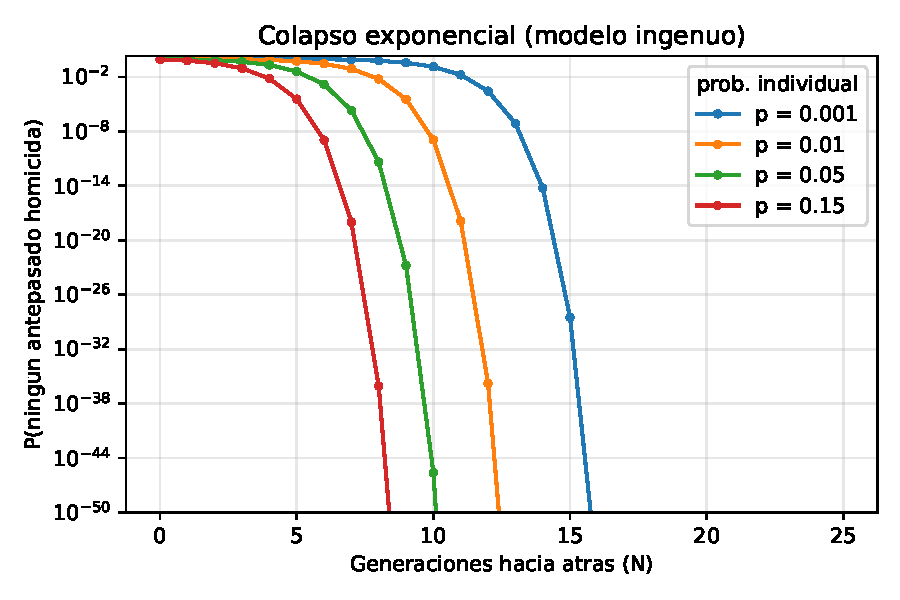
\includegraphics[width=0.72\textwidth]{fig_naive_collapse.pdf}
\caption{Colapso exponencial de $P_{\text{ing}}(p,N)$ (escala logar\'itmica)
seg\'un el modelo ingenuo, Ec.~\eqref{eq:naive}.}
\label{fig:naive}
\end{figure}

\begin{figure}[h]
\centering
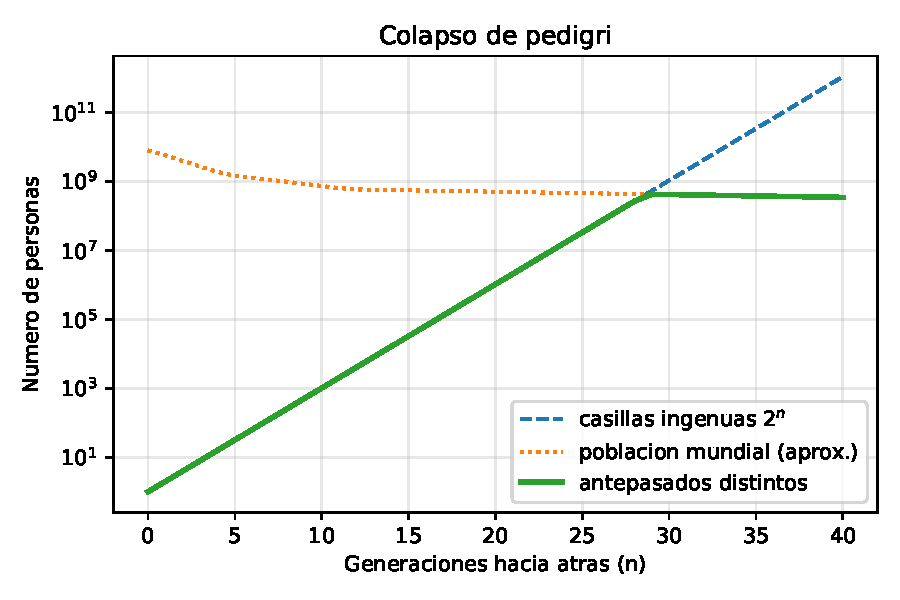
\includegraphics[width=0.72\textwidth]{fig_pedigree_collapse.pdf}
\caption{Colapso de pedigr\'i: las casillas ingenuas $2^n$ superan a la
poblaci\'on, por lo que los antepasados distintos $D(n)$ saturan,
Ec.~\eqref{eq:collapse}.}
\label{fig:collapse}
\end{figure}

\begin{figure}[h]
\centering
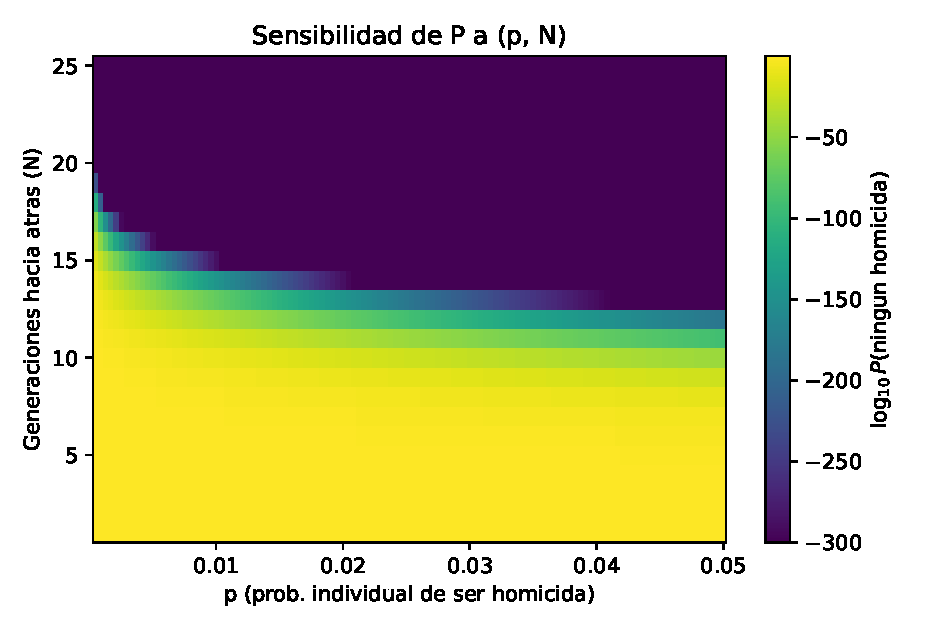
\includegraphics[width=0.72\textwidth]{fig_sensitivity_heatmap.pdf}
\caption{Sensibilidad de $\log_{10} P_{\text{ing}}$ a $(p,N)$. La regi\'on
oscura (probabilidad $\approx 0$) domina salvo para $p$ muy peque\~no y $N$ muy
peque\~no.}
\label{fig:heat}
\end{figure}

\section{Discusi\'on y limitaciones}\label{sec:disc}

\paragraph{Independencia.} La hip\'otesis de independencia es falsa: la
propensi\'on a la violencia correlaciona dentro de familias y regiones, y los
eventos b\'elicos afectan a muchos a la vez. Sin embargo, la correlaci\'on
positiva tiende a \emph{reforzar} la conclusi\'on (concentra homicidas en
algunas ramas, pero basta una rama para romper la conjunci\'on), y la simulaci\'on
con emparejamiento aleatorio ya prescinde de la poblaci\'on infinita.

\paragraph{Geneal\'ogico vs.\ gen\'etico.} El argumento es \emph{geneal\'ogico}.
Un antepasado del IAP puede no haber dejado material gen\'etico en \emph{ego}
\citep{ralph2013}. Esto no afecta la afirmaci\'on sobre descendencia, que es de
\'indole geneal\'ogica, no gen\'etica.

\paragraph{Sensibilidad a la definici\'on.} Con una definici\'on legal estricta
de ``asesinato'' (homicidio il\'icito), $p$ ser\'ia menor; aun as\'i, las
Tablas~\ref{tab:iap} y~\ref{tab:sim} muestran que el resultado se mantiene para
$p$ tan bajos como $10^{-4}$.

\paragraph{Mezcla poblacional.} El modelo de \citet{rohde2004} asume mezcla
global, mitigada en la realidad por barreras geogr\'aficas; esto retrasa el IAP
global pero no lo elimina, y el IAP \emph{regional} es a\'un m\'as reciente.

\paragraph{Posicionamiento y novedad.} Este trabajo no reclama un resultado
matem\'atico nuevo: es una \emph{s\'intesis} expositiva que combina resultados
ya conocidos ---la ascendencia com\'un reciente de \citet{chang1999} y
\citet{rohde2004}, y la prevalencia de violencia letal de \citet{gomez2016}---
para responder de forma cuantitativa a una pregunta existencial concreta. Su
aporte es pedag\'ogico y de integraci\'on: hace expl\'icito, con c\'odigo
reproducible y an\'alisis de sensibilidad, un corolario que suele permanecer
impl\'icito en la literatura de genealog\'ia gen\'etica.

\section{Conclusi\'on}

La probabilidad de no tener ning\'un antepasado homicida es, bajo cualquier
parametrizaci\'on realista, indistinguible de cero. El crecimiento exponencial
de antepasados y el colapso de pedigr\'i bastan para hacerla \'infima en pocas
generaciones; el punto de ancestros id\'enticos la convierte en una certeza
pr\'actica de car\'acter casi deductivo. Por tanto, \emph{es esencialmente
imposible que un ser humano vivo no descienda de al menos un homicida}. La
intuici\'on existencial que motiv\'o esta nota queda, as\'i, rigurosamente
refutada.

\section*{Reproducibilidad}
\addcontentsline{toc}{section}{Reproducibilidad}
Todos los resultados num\'ericos, tablas y figuras se generan con el c\'odigo en
el directorio \texttt{code/} (Python; v\'ease \texttt{requirements.txt}). La
simulaci\'on Monte Carlo usa semillas fijas, de modo que sus resultados son
deterministas y reproducibles. El presente documento se compila con Tectonic
(\texttt{tectonic main.tex}).

\section*{Disponibilidad de datos y c\'odigo}
\addcontentsline{toc}{section}{Disponibilidad de datos y c\'odigo}
El c\'odigo, los datos derivados y las fuentes de este art\'iculo est\'an
disponibles en el repositorio del proyecto
(\url{https://github.com/JuanoLemos/paper-antepasado-asesino})% TODO(Fase C): fijar URL/DOI definitivos
\ y se archivar\'an con un DOI permanente en Zenodo. La trazabilidad de cada
afirmaci\'on a su fuente primaria se documenta en el archivo
\texttt{EVIDENCE.md}. El c\'odigo se distribuye bajo licencia MIT y el texto y
las figuras bajo CC-BY-4.0.

\section*{Conflicto de inter\'es}
\addcontentsline{toc}{section}{Conflicto de inter\'es}
El autor declara no tener conflictos de inter\'es.

\bibliographystyle{plainnat}
\bibliography{refs}

\end{document}
